\newpage
%\section{Introduction}
\chapter{Introduction}
Schizophrenia is a psychotic disorder where at least two of the symptoms delusions, hallucinations, disorganized speech, grossly disorganized or catatonic behaviour or negative symptoms such as reduced emotional expressions and lowered motivation, have to be present. 
Delusions are beliefs that will not change if contradicting evidence is presented. The most common type of delusions are persecutory delusions. People that have those kinds of delusions might think that they will be hurt, injured, tormented or so on by others. Referential delusions are also common. Then one are putting meaning into comments, gestures and actions, thinking that they are about oneself, when they not necessarily are. Completely improbable beliefs are called bizarre delusions. These are delusions others find far-fetched, and they are things that cannot happen in real life. A bizarre delusion could for example be that a person believes that their organs have been removed replaced by someone else's organs without there being any scars or other evidence of that happening. A delusion that is not bizarre could be that you think you are under police surveillance without there being any evidence of that. It might be hard to distinguish between delusions and strongly held ideas. The main distinction is about the degree of conviction, and how much or little the beliefs can be amended when contradicting facts are presented \citep{dsm-5}. 
%Hallucinations are sensory impressions that happen without any external stimulus. Hence, others usually does not experience the same impressions. The hallucinations are perceived as normal experiences to the person having them. For schizophrenic people, they often occur as voices which can be distinguished from the persons own thoughts. 
%Disorganized speech means that one are switching between topics rapidly and giving unrelated answers to questions. 
%Grossly disorganized behavior is also referred to as abnormal behavior, and catatonic behavior means that one has a dampened reaction to things happening around oneself. (All of the above is from DSM-5).


Delusions are one of the main characteristics of schizophrenia as it appears in about three out of four of those diagnosed \citep{garety2011}. Researchers have been trying to understand how the delusions are formed and maintained in order to improve treatment \citep{dudley_meta_2016}. One important finding is that deluded individuals seem to make decisions based on less evidence than both healthy and psychiatric controls. This is often referred to as a "jumping to conclusions" (JTC) bias. A person with this bias might reach decisions or form beliefs before reaching realistic conclusions, and thus accept unrealistic ideas. They are therefore more prone to delusions. The hope is that if we can detect the JTC bias, we can reduce the delusional thinking, and thus prevent delusions.

The JTC bias is traditionally tested with a probabilistic reasoning task called the beads task. The participants are presented with two jars containing beads of two colours, for example red and blue. The two jars have opposite ratios of each colour, meaning that if the first have 85\% red beads and 15\% blue, the second has 15\% red and 85\% blue beads. The participants are told that beads are drawn from one of the jars, and their task is to find out which one that is. They are told to choose only when they are completely sure, and they draw as many beads as they want. The beads are drawn sequentially, and after each draw the participants are asked if they want to choose which jar beads are drawn from or if they want to draw more beads. One are usually said to have a JTC bias if one decides after one or two beads \citep{moritz2017}. However, the beads task has shown to pose some problems.

Some of the first to use the beads task were \citet{huq1988}. Already in that article they presented some of the problems with the beads task. They used an 85-15 ratio of the beads. When the two first beads that are drawn are of the same colour, it is a 97\% probability that the beads are from the jar with 85\% of the beads in that colour. One might therefore argue that choosing jar at that point is reasonable, and that it does not show a JTC bias. Deluded individuals make decisions earlier that the control groups, but \citeauthor{huq1988} argue that non-deluded individuals are more conservative, and that people with delusions simply cancel out that bias when gathering less information. In an article by \citet{moritz2017}, other problems with the beads task are discussed. For example that many participants seem not to understand that all the beads are drawn form the same jar. This makes them think that after each bead is drawn, they have to guess which jar that bead is drawn from. These participants are then classified to have a JTC bias. We can also see that it is common to make logical errors due to miscomprehension. In an article by \citet{moritz2005}, they found that 52\% of the schizophrenic participants and 23\% of the healthy controls had at least one response that was not logical. The participants that misunderstand are more likely to choose early. \citet{moritz2017} further states that the beads task is correlated with intelligence. Lack of intelligence might be a reason for or a confound for misunderstanding the task. It is also stated that confidence influences decision-making. The participants are asked to choose when they are completely sure which jar the beads are drawn from, which could make more confident participants decide earlier. We might also conclude that hasty decisions are made because the participants like to take risks or that they are not cautious, or both. However, other tasks that accounts for confidence also display a JTC bias with the delusion-prone participants. Additionally, there is only a one-dimensional sequence of events in the beads task. Thus, it is harder to find different versions to test multiple times. 

The box task has been suggested as an alternative to the beads task. Here, the participants are presented with a grid of a fixed number of boxes. When a box is opened, one out of two colours is displayed, for example blue and red. The participants are told that one of the colours always is in majority, and their task is to find out which one \citep{moritz2017}. They can open as many boxes as they want before making a decision. Both the number of boxes and the ratio of the two colours can be changed for each new trial. 

In this report we model how the participants make decisions in the box task. In the version of the box task used here, there are twelve boxes. We use two different versions of the box task. The first is an unlimited one, where the participants can open as many boxes as they want, even until all twelve boxes are opened, before reaching a decision. In the second version, the participants are told that the test will terminate at a random point. If the test terminates before the participant has decided what the majority colour is, this counts as a failed trial. We call this the limited version. In Figure \ref{picture_of_box_task}, we see a limited trial of the box task with red and blue boxes. The participant has opened two boxes, and has to choose whether to open another box or to choose that either blue is the dominant colour, or that red is. 
\begin{figure}
    \centering
    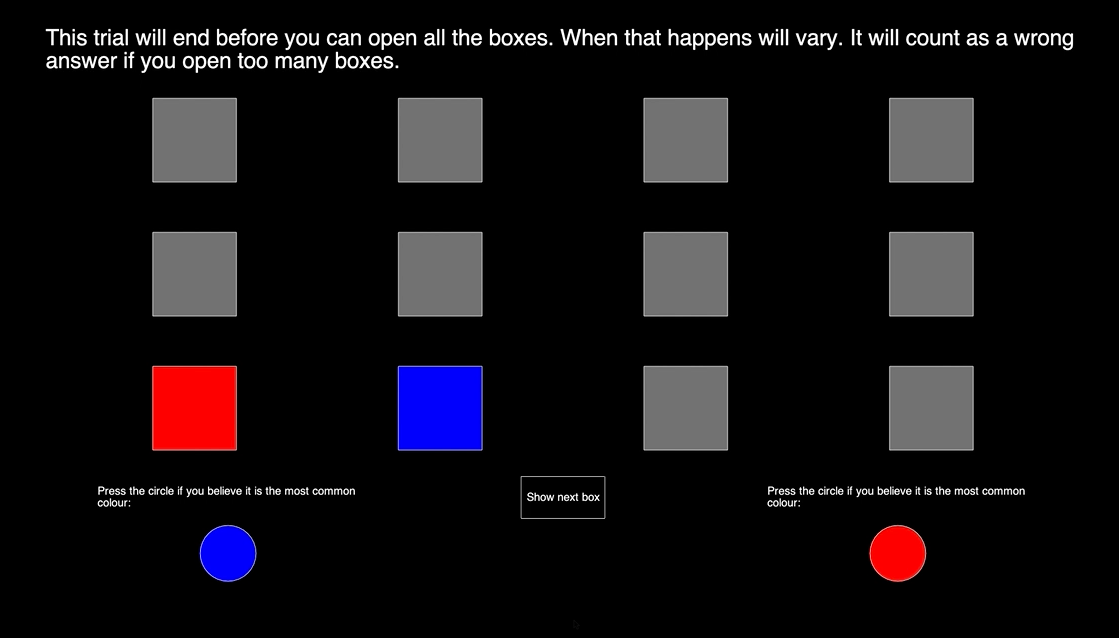
\includegraphics[scale=0.486]{Sections/Box task 2.png}
    \caption[A Limited Trial of the Box Task Visualised]{A limited trial of the box task with two opened boxes. The participants are to find out what the majority colour is given that one of them always is in majority.}
    \label{picture_of_box_task}
\end{figure}

We have data from 76 participants that have done 10 trials each of the box task. The first trial was a practice trial of the limited version followed by three unlimited and six limited trials. We can model the decisions the participants make using a softmax model, and fit this model to each participant with maximum likelihood estimation. Thus, we find the maximum likelihood estimates in the softmax model. We then find confidence intervals for each of these estimates using parametric bootstrapping and percentile intervals. 

As an input in the Softmax model we have an Ideal Observer solution of the box task. An Ideal Observer is a participant that always makes optimal, or ideal, choices, and thus finds the best solution \citep{idealObs}. Each time a box is opened, the participant have three options. The first is to choose that blue is the majority colour, the second that red is, and the third option is to open another box. For each of these alternatives we have defined loss functions, which represent the cost of choosing the different options. An Ideal Observer would always choose the alternative with the least expected loss, and would end up with the overall optimal, or ideal, solution. In this report we are assuming that the total number of red boxes is binomially distributed with parameters 12 and some probability $\theta$. Each time a box is opened, the probability that the box is red is $\theta$ and $1-\theta$ that the box is blue. We also assume a beta prior for $\theta$ with parameters $\gamma$ and $\kappa$. If we have any prior beliefs about the probability of the different colours, this knowledge can be incorporated here. If both $\gamma$ and $\kappa$ are one, this is a uniform prior, meaning that $\theta$ has the same probability of being each possible value between zero and one. 



%(something about: here they are not said to answer when they are completely sure? compared to the beads task, where they are said to answer when comp sure. Jeg klarer ikke å finne ut hvor det står??)


In this report we will firstly go through some of the background theory used later on. Then, we will formulate the model for the decisions the participants make. That includes finding an Ideal Observer solution of the box task, and describing how to find parameter estimates and confidence intervals. Further on we will present some results, both the Ideal Observer solution and the parameter estimated with their respective confidence intervals. Lastly, we have some closing remarks. 